\documentclass{article}
\usepackage{tikz}
\usetikzlibrary{through,shapes}

\begin{document}
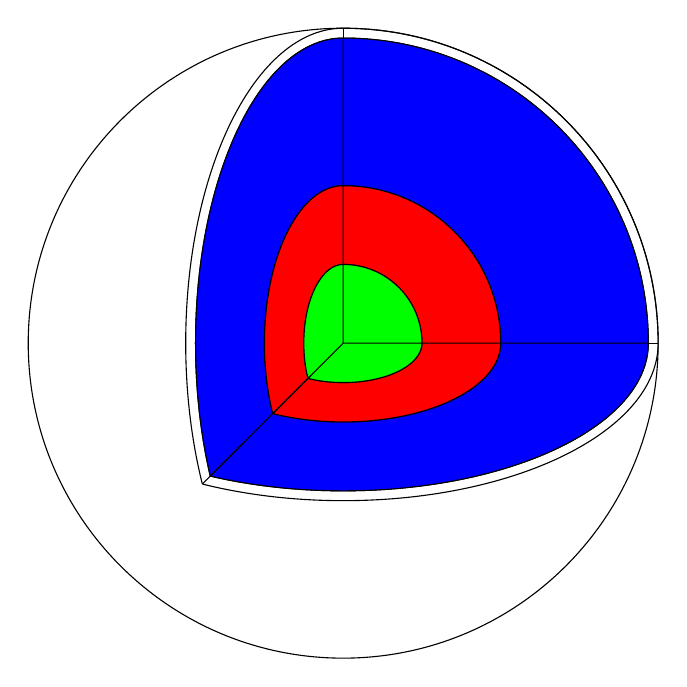
\begin{tikzpicture}
    % coordinaten
    \coordinate (m) at (0,4,0);
    % assen
    \draw (0,0,0) -- (0,4,0); % z
    \draw (0,0,0) -- (4,0,0); % x
    \draw (0,0,0) -- (0,0,4.65); % y
    % sfeer
    \draw (4,0,0) arc (0:116.5:4cm and -2cm);
    \draw (4,0,0) arc (0:90:4cm and 4cm);
    \draw (0,4,0) arc (90:206.5:2cm and 4cm);
    \node[draw,circle through={(m)}] (c) at (0,0,0) {};
    % fotosfeer
    \draw (3.875,0,0) arc (0:115.8:3.875cm and -1.875cm);
    \draw (3.875,0,0) arc (0:90:3.875cm and 3.875cm);
    \draw (0,3.875,0) arc (90:205.8:1.875cm and 3.875cm);
    %fill
    \draw[fill=blue] (0,0,0) --(0,3.875,0) arc (90:205.8:1.875cm and 3.875cm) 
--(0,0,0) -- (3.875,0,0)  arc (0:90:3.875cm and 3.875cm) -- (0,0,0) -- 
(3.875,0,0) arc (0:115.8:3.875cm and -1.875cm)--  cycle;
    % convenctie zone
    \draw (2,0,0) arc (0:116.5:2cm and -1cm);
    \draw (2,0,0) arc (0:90:2cm and 2cm);
    \draw (0,2,0) arc (90:206.5:1cm and 2cm);
    %fill
    \draw[fill=red] (0,0,0) -- (0,2,0) arc (90:206.5:1cm and 2cm) --(0,0,0) -- 
(2,0,0)  arc (0:90:2cm and 2cm) -- (0,0,0) -- (2,0,0) arc (0:116.5:2cm and 
-1cm)--  cycle;
    % radiatie zone
    \draw (1,0,0) arc (0:116.5:1cm and -0.5cm);
    \draw (1,0,0) arc (0:90:1cm and 1cm);
    \draw (0,1,0) arc (90:206.5:0.5cm and 1cm);
    %fill
    \draw[fill=green] (0,0,0) -- (0,1,0) arc (90:206.5:0.5cm and 1cm) --(0,0,0) 
-- (1,0,0)  arc (0:90:1cm and 1cm) -- (0,0,0) -- (1,0,0) arc (0:116.5:1cm and 
-0.5cm)--  cycle;

\end{tikzpicture}
\end{document}
